
\section{Introducción}

En este capítulo se definen algunos conceptos importantes sobre comprensión de programas (CP).
La CP es un área de la Ingeniería de Software que tiene como meta primordial desarrollar métodos, técnicas y herramientas que ayuden al programador a comprender en profundidad los sistemas de software. 

Diversos estudios e investigaciones demuestran que el principal desafío en la CP es vincular el \textit{Dominio del Problema} y el \textit{Dominio del Programa} \cite{BRM10,MPMR07,MBPHRU10,DWE04}. El primero se refiere al resultado de la ejecución del sistema, mientras que el segundo indica todos los componentes de software que causaron dicho resultado. 

La comunidad de CP sostiene, basado en estudios de los modelos cognitivos, que un programador entiende un programa cuando puede relacionar el comportamiento del mismo con su operación. En otras palabras cuando puede vincular el \textit{Dominio del Problema} y el \textit{Dominio del Programa}. El inconveniente es que este vínculo es complejo de llevar a cabo, por ende se puede bosquejar una aproximación a través de los siguientes pasos: I) Elaborar una representación para el Dominio del Problema; II) Construir una representación del Dominio del Programa y III) Elaborar un procedimiento de vinculación. La Figura \ref{captura1} muestra un modelo de comprensión que refleja lo mencionado previamente.

\begin{figure}[t] %[h] para here [b] para bottom [t] para top
\centerline{%queda centrada mejor la imagen
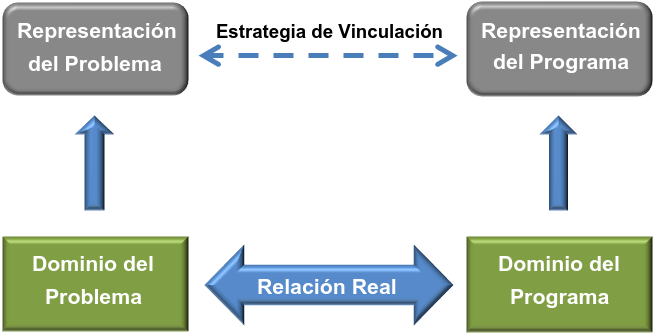
\includegraphics[scale= 0.7]{./cap2/dom.png}
}
\caption{Modelo de Comprensión de Programas}
\end{figure} \label{captura1}
 
Para lograr con éxito los pasos antedichos se deben tener en cuenta conceptos muy importantes que son los cimientos sobre los cuales está sustentada la CP: los \textit{modelos cognitivos}, la \textit{extracción de información}, la \textit{administración de la información}, la \textit{visualización de software} y la \textit{interconexión de dominios}. Estos conceptos fueron descriptos brevemente en el capítulo anterior, a continuación se desarrolla una explicación más amplia de cada uno.

\section{Modelos Cognitivos}

Los \textit{Modelos Cognitivos} se refieren a las estrategias de estudio y las estructuras de información usadas por los programadores para comprender los programas \cite{TIE89,VMAVA95,BROOK82,STOREY99}. Estos modelos  son importantes porque indican de que forma el programador comprende los sistemas y como incorpora nuevos conocimientos (en términos generales aprende nuevos conceptos).
Los Modelos Cognitivos están compuestos por: \textit{Conocimientos}, \textit{Modelos Mentales} y \mbox{\textit{Procesos de Asimilación} \cite{MBPHRU10}.} Estos conceptos se detallan a continuación.

\begin{description}

\item[Conocimiento:] Existen dos tipos de conocimientos, por un lado está el conocimiento interno el cual se refiere al conocimiento que el programador ya posee antes de analizar el código del sistema de estudio. Por otro lado existe el conocimiento externo que representa un soporte de información que le brinda al programador nuevos conceptos. Este conocimiento externo es el que proporciona el sistema que se quiere entender, con todos los artefactos asociados al mismo.
Los ejemplos más comunes son la documentación del sistema, otros desarrolladores que conocen el dominio del problema, códigos de otros sistemas con similares características, entre otras tantas fuentes de información.

\item[Modelo Mental:] Este concepto hace referencia a representaciones mentales que el programador elabora al momento de estudiar el código del sistema. 
%Estas representaciones mapean a distintas componentes del sistema. 
Algunos ejemplos de modelos mentales son: el grafo de llamadas a funciones, el grafo de dependencias de módulos, diagramas de flujo, etc. Es importante mencionar que algunos modelos mentales permiten una representación visual que posibilita que dicho modelo sea exteriorizado. Esta demás decir que esta característica ayuda al programador a entender un programa.

\item[Proceso de Asimilación:] Está compuesto por estrategias de aprendizaje que el programador usa para llevar adelante la comprensión de un programa. Los procesos de asimilación se pueden clasificar en tres grupos: Bottom-up, Top-Down e Híbrido \cite{MPOB03,MAS05}. A continuación se explica cada uno.

\begin{description}

\item[Bottom-up:] El proceso de comprensión \textit{Bottom-up}, indica que el desarrollador primero lee el código del sistema. Luego, mentalmente las líneas de código leídas se agrupan en distintas abstracciones de más alto nivel. Estas abstracciones intermedias se van construyendo hasta lograr una abstracción comprensiva total del sistema.

\item[Top-down:] Brooks explica el proceso teórico \textit{top-down}, donde el programador primero elabora hipótesis generales del sistema en base a su conocimiento del mismo. En ese proceso se elaboran nuevas hipótesis las cuales se intentan validar y en ese proceso se generan nuevas hipótesis.
%Luego estas hipótesis generales son comprobadas y refinadas a nuevas hipótesis más detalladas. Estas hipótesis nuevas también son comprobadas y generan nuevas hipótesis.
Este proceso se repite hasta que se encuentre un trozo de código que implementa la funcionalidad deseada.

Para resumir, el proceso de aprendizaje bottom-up procede de lo más específico (código fuente) a lo más general (abstracciones). Mientras que el top-down es a la inversa.

\item[Híbrido:] Este proceso combina los dos conceptos mencionados anteriormente \textit{top-down} y \textit{bottom-up}. Durante este proceso de aprendizaje del sistema, el programador combina libremente ambas políticas (\textit{top-down} y \textit{bottom-up}) hasta lograr comprender el sistema.
\end{description}
\end{description}

%Por otro lado el modelo de comprensión top-down es una estrategia en donde primero el programador usa el conocimiento adquirido del dominio del problema para construir perspectivas del sistema en forma de modelo y luego estas perspectivas se vinculen con los distintos fragmentos del código.

La teoría descripta en esta sección sobre Modelos Cognitivos, marca la importancia de esta temática en el ámbito de la CP y de lo difícil que es desarrollar métodos, técnicas y herramientas en este ámbito.

Para llevar a cabo estrategias involucradas en Modelos Cognitivos, es importante extraer información desde los códigos de estudio, en el próximo apartado se hace hincapié en este tema.
%Para concluir sobre la temática de modelos cognitivos: el modelo mental es una representación mental que el programador tiene sobre el sector del sistema que esta analizando. Si esta representación se la vincula con los conocimientos que el propio programador posee, se logra un entendimiento de esa parte del sistema, como así también incrementa los conocimientos del programador. Con esto se deja en claro la importancia de modelos cognitivos en el proceso de entendimiento de los sistemas.%CONSULTAR

\section{Extracción de Información}

En la Ingeniería del Software existe un área que se encarga de la \textit{Extracción de la Información} desde los sistemas se software. 
%Esta extracción se realiza en los sistemas de software y las técnicas utilizadas para tal fin, se clasifican según el tipo de información que extraen. 
Existen dos tipos de informaciones: la Estática y la Dinámica. A continuación se explica cada una y se da un ejemplo de como pueden ser extraídas desde los programas.

\begin{description}
\item[Información Estática:] Está presente en los componentes del código fuente del sistema. Alguno de ellos son identificadores, procedimientos, comentarios, documentación.
Una forma para extraer la información estática consiste en utilizar técnicas tradicionales de compilación \cite{AHUL06}. Estas 
técnicas, utilizan un analizador sintáctico similar al empleado por un compilador. Este analizador sintáctico, por medio de acciones semánticas específicas procede a capturar elementos presentes en el código durante la fase de compilación. En la actualidad, existen herramientas automáticas que ayudan a construir este tipo de analizador sintáctico.

%Otra estrategia de extracción de información estática es la vista de grafo de llamadas a funciones\cite{MBPHRU10}. Las aristas de este grafo son funciones del programa de estudio y los arcos representan las llamadas entre dos funciones. Esta vista permite observar la invocación entre funciones. Utiliza la relación llamador-llamado en base solo al código fuente. Simplemente se colocan sentencias en el código indicando desde donde se invocan las funciones. Con esto se sabrá quien llama a una determinada función para llevar a cabo la construcción del grafo.

%Ambas estrategias estáticas descriptas no requieren ejecutar el sistema de estudio.

%Para construir el analizador se suele utilizar una herramienta automatizada que lee una gramática y después genera el parser. En esta gramática asociada a un lenguaje particular se insertan acciones semánticas que formarán parte del parser generado.
%Otra forma es usando grafo de llamadas a funciones en donde las aristas son funciones del programa de estudio y los arcos representan las llamadas entre dos funciones. A nivel conceptual es fácil de entender pero a veces la complejidad de los sistemas impiden una ágil realización sobre todo si los bloques de código tienen una complejidad temporal y espacial con cotas elevadas \cite{MBPHRU10}. Para la construcción de este grafo no se necesita ejecutar el programa.

\item[Información Dinámica:] Se basa en elementos del programa presentes durante una ejecución específica del sistema \cite{THBE99}. Un ejemplo conocido de una técnica que extrae información dinámica es la instrumentación de código. Esta técnica inserta sentencias nuevas en el código fuente. La finalidad de las nuevas sentencias es registrar las actividades realizadas durante la ejecución del programa. 
%Para la extracción de este tipo de información se procede a bosquejar una técnica de instrumentación de código la cual consiste en insertar sentencias en el código sin modificar su semántica, así cuando el sistema se ejecute estas sentencias que contienen acciones se van a encargar de indicar que operaciones internas se llevaron a cabo para una determinada salida del programa.
Estas sentencias nuevas no deben modificar la funcionalidad original del sistema, por ende la inserción debe realizarse con sumo cuidado y de forma estratégica para no alterar el flujo normal de ejecución.

\end{description}

Tanto las estrategias de extracción de información estáticas, como las dinámicas son importantes ya que permiten elaborar técnicas para comprender programas. A veces, se recomienda complementar el uso de ambas estrategias para obtener mejores resultados, sobre todo si el sistema que se está analizando es grande y complejo \cite{TERD01}.

%La extracción de información cumple un rol fundamental en la CP. Como se explicó antes, en la CP se destaca la relación entre el dominio del problema y el dominio programa, como esta relación es compleja, se elabora una aproximación mediante el uso de representaciones (ver figura \ref{captura1}). Necesariamente, para poder bosquejar dichas representaciones se debe extraer información de ambos dominios.

Cabe destacar que extraer información de los sistemas implica tomar ciertos recaudos. Si la magnitud de información es demasiado grande se puede dificultar el acceso y el almacenamiento de la misma. Es por esto que se recurre a las técnicas de administración de información. En la próxima sección se explica con más detalles esta afirmación.

%Otra forma de extraer información dinámica, es usando un árbol de ejecución de funciones\cite{MBPHRU10}. Para armar esta estructura se necesita insertar sentencias en el código que señalen el inicio y fin de cada función. El orden en el que se ejecutan estas sentencias para una ejecución particular se resguardan en una pila, luego la pila es leída y el árbol se construye. Esta gráfica clarifica las llamadas que se hicieron entre funciones para una corrida particular.

%Los párrafos anteriores permiten percibir la importancia de las las técnicas de extracción de información estáticas y dinámicas. Sin estas técnicas sería imposible construir estrategias de comprensión de programas. Más precisamente, se necesitan para extraer información de los 2 dominios antedichos, el del problema y del programa (ver figura \ref{captura1}).

%Una vez extraída la información, la misma se recomienda que sea administrada.

%Volviendo al objetivo principal que es aproximarse en la construcción de relación del dominio del problema con el dominio programa a través de representaciones esta requiere la extracción de información de ambos dominios.

%La extracción de información del dominio del programa es una metodología sencilla de llevar a cabo por el hecho de que su extracción está claramente marcada. El inconveniente radica en la extracción de la información perteneciente al dominio del problema, porque esta información es sensible a las características propias de la aplicación. Para encarar este inconveniente la ingeniería del software propone tomar las fuentes de información informal las cuales pueden estar presentes en el código por ejemplo: comentarios, literales string; o fuera del mismo: documentación, entrevistas con el cliente etc. Un vez que se extraen estos componentes se les puede aplicar alguna técnica de análisis de información informal para interpretar algunas las funcionalidades de los componentes del sistema.

%Hasta aquí solo se ha mencionado estrategias de extracción información de los dominios del problema y del programa. Desafortunadamente el mapeo que relaciona la salida del sistema con los componentes que la integran queda a manos del programador y no abundan herramientas automatizadas que simplifiquen esta tarea.

\enlargethispage{\baselineskip}%agrega linea al final de la hoja
\section{Administración de la Información}

Teniendo cuenta que lo sistemas son cada vez más amplios y complejos. El volumen de la información extraída de los sistemas crece notoriamente, por lo tanto se necesita administrar la información.

Las técnicas de \textit{Administración de Información} se encargan de brindar estrategias de almacenamiento y acceso eficiente a la información recolectada de los sistemas. 

Dependiendo del tamaño de la información se utiliza una determinada estrategia. Estas estrategias indican el tipo de estructura de datos a utilizar y las operaciones de acceso sobre ellas \cite{AAJU83,TSTA80}. La eficiencia en espacio de almacenamiento y tiempo de acceso son claves a la hora de elegir una estrategia.
Cuando la cantidad de datos son de gran envergadura, se recomienda emplear una base de datos con índices adecuados para realizar las \mbox{consultas \cite{ERNS99}.}

Después que se administra la información, se aconseja que la misma sea representada por alguna técnica de visualización. Esta representación, permite esclarecer la información del sistema de una mejor manera para que sea interpretada por el programador. El área encargada de llevar adelante esta tarea es la Visualización de Software.

%Una temática importante en las técnicas explicadas SVS, BORS y SVSI es la visualización de software. En la siguiente sección se explica este punto.

\enlargethispage{\baselineskip}%agrega linea al final de la hoja

\section{Visualización de Software}

La \textit{Visualización de Software} es una disciplina de la Ingeniería del Software. Esta disciplina, se encarga de visualizar la información presente en los programas, con el propósito de facilitar el análisis y la comprensión de los mismos. Esta cualidad es interesante ya que en la actualidad los sistemas son cada vez más amplios y complicados de entender. Esta disciplina además brinda apoyo en lo que respecta a la comprensión de las distintas etapas involucradas en el desarrollo de los sistemas, como es el caso del análisis, diseño, implementación y mantenimiento \cite{MBPHRU10}. Por ende, la Visualización de Software colabora en la CP.

Para lograr lo descripto en el párrafo anterior, la Visualización de Software provee distintos sistemas de visualización. Estos sistemas son herramientas útiles que se encargan de analizar los distintos módulos de un programa y generar vistas. Las vistas son una representación visual de la información contenida en el software. Generalmente, una herramienta de comprensión de programas posee varias vistas que ayudan a comprender un programa, dependiendo de la información que se requiera visualizar existe una vista adecuada a cada caso. Las vistas en el contexto de la CP, representan puentes cognitivos que achican la brecha entre los conocimientos del programador y los conceptos usados en el software de estudio.

Para concluir, el objetivo primordial de la visualización de software orientada a la CP es generar vistas (representaciones visuales), que ayuden a reconstruir el vinculo entre el Dominio del Problema y el Dominio del Programa. De manera más sencilla, el objetivo es representar visualmente la salida del sistema, los componentes utilizados para dicha salida y la relación que existe entre ambos.

%Esto permite, interpretar los programas de manera más clara y ágil. Dependiendo de la información que se desea visualizar existe una vista específica \cite{MPMR07}.

%De esta manera, facilita las tareas de mantenimiento al programador, sobre todo, en sistemas amplios y complicados. 

%Las vistas cuando están bien construidas clarifican más la comprensión del sistema.


%Cabe recordar que la información concebida en un sistema puede ser estática o dinámica. 

%Existen distintos tipos de vistas, en si mismo, la primer vista de un sistema es el código en donde la información no está tan clara para un desarrollador ajeno sobre todo si el software es grande y complicado.

%Es por eso que se necesita recurrir a otras vistas que representen una abstracción mas clara del sistema.
 
%Las vistas poseen distintas características y para su construcción se requieren un conjunto de librerías gráficas. Dichas librerías son programas que simplifican la elaboración de las vistas y el diseñador de la visualización tiene la tarea de elegir que librería es la más adecuada para la vista que desea construir. Las librerías gráficas mas conocidas son Jung, Prefuse, Graphviz y Cairo \cite{BRM10}.

%En la actualidad, existen distintas taxonomías sobre la visualización del software, algunos de los autores son: Myers, Price, Roman, Kenneth, Storey \cite{MBPHRU10}. Sin embargo, todos estos sistemas de visualización tienen algo en común, las vistas que son generadas por estos sistemas, representan conceptos situados solo en el dominio del programa, restando importancia al dominio del problema y a la relación entre ambos dominios.

%Debido a esta falencia Berón \cite{MBPHRU10} propone variantes en los sistemas de visualización orientados a la CP. Estas variantes contemplan la representación visual de los conceptos en el dominio del problema, inclusive la visualización de la relación entre los dos dominios mencionados.


\pagebreak
\section{Estrategias de Interconexión de \\Dominios}

Los conceptos explicados en los puntos anteriores como la \textit{visualización de software} y la \textit{extracción de la información} forman la base para elaborar estrategias de interrelación de dominios.

La \textit{Interconexión de Dominios} en la Ingeniería del Software, tiene como objetivo principal la transformación y vinculación de un dominio específico en otro dominio. Este último dominio puede estar en un nivel más alto o más bajo de abstracción. Lo primordial aquí, es que cada componente de un dominio se vea proyectado en uno o más componentes de otro dominio y viceversa.

%Cuando se dice que relacionar el dominio del problema con el dominio del programa es importante ya que permite al desarrollador encontrar de forma mas ágil y rápida componentes en el software para una operación específica. Esto facilidad impacta directamente en los tiempos dedicados a la evolución y al mantenimiento del software por el simple hecho de que se reduce la ardua tarea que tiene el programador de comprender el código.
%Sin embargo, solo se podrá destacar este impacto si el software de estudio es muy amplio y complejo.

Un ejemplo sencillo de \textit{Interconexión de Dominios}, es cuando el dominio del código fuente de un programa, se puede transformar en un Grafo de Llamadas a Funciones (Dominio de Grafos). Cada nodo del grafo representa una función particular y cada arco las funciones que puede invocar. En este ejemplo la relación entre ambos dominios (código y grafo) es clara y directa. 

Es importante aclarar que existe una amplia gama de transformaciones entre dominios. La más escasa y difícil de conseguir es aquella que relaciona el Dominio del Problema con el Dominio del Programa (Ver Figura \ref{captura1}).

Sin embargo, actualmente existen técnicas recientemente elaboradas, que conectan visualmente el Dominio del Problema y el Dominio del Programa mediante la información estática y dinámica que se extrajo del sistema de estudio, algunos ejemplos son \textit{Simultaneous Visualization Strategy} (SVS), \textit{Behavioral-Operational Relation Strategy} (BORS) y \textit{Simultaneous Visualization Strategy Improved} (SVSI) \cite{BRM10,MPMR07,MBPHRU10}. Estas técnicas son muy útiles para la CP, ya que diagraman la salida del sistema con los componentes que intervinieron  en dicha salida.

%Una de las técnicas es \textit{Simultaneous Visualization Strategy} SVS, esta se encarga de mostrar los distintos componentes de un programa en plena ejecución, mediante distintas vistas, usando un inspector de sentencias, de esta manera se obtiene una visualización cuando el sistema se está ejecutando. Esta estrategia usa un esquema de instrumentación de código, donde las acciones semánticas le van indicando a un visualizador la traza de invocaciones a funciones durante la ejecución del sistema \cite{BRM10,MPMR07,MBPHRU10}.

%La otra estrategia se denomina \textit{Behavioral-Operational Relation Strategy} BORS, que a diferencia del SVS, espera a que termine la ejecución del sistema y luego la información recopilada por el instrumentador de código es procesada por BORS. Una vez procesada la información, BORS retorna una abstracción gráfica del código ejecutado. BORS vincula los conceptos del código capturados en tiempo de ejecución con la información asociada al dominio del problema \cite{BRM10,MPMR07,MBPHRU10}.

%Existe también, a nivel conceptual una técnica que combina ambas estrategias mencionadas llamada \textit{Simultaneous Visualization Strategy Improved} SVSI. Esta técnica disminuye los problemas que manifiestan tanto SVS como BORS y con ello se logra un mejor desempeño en cuanto a los resultados esperados \cite{BRM10,MPMR07,MBPHRU10}.

\pagebreak
\section{Notas y Comentarios}

Para resumir las ideas tratadas en este capítulo, el área de la CP le da mucha importancia a la relación entre el \textit{Dominio del Problema} y el \textit{Dominio del Programa}. Esta relación es clave, por que ayuda al programador a entender con facilidad los programas, ya que encuentra las partes del sistema que produjeron una determinada salida. Dado que los especialistas determinan que es complicado este vínculo \cite{AMPM11,MPMR07,MBPHRU10,DWE04}, un camino para aproximarse a la difícil solución de unir ambos dominios, es construir una representación de cada uno y luego unirlos con una estrategia de relación. Para llevar a cabo estos pasos, se necesitan estudiar las temáticas pertinentes: los \textit{modelos cognitivos}
indican como el programador emplea procesos mentales para comprender el sistema; para implementar estos modelos se necesita \textit{extraer información} del software de estudio; si esta información es mucha se recomienda \textit{administrar la información}; generalmente esta información extraída de los sistemas, es más fácil de interpretarla si se emplea la \textit{visualización de software}; por último la \textit{interconexión de dominios} es una pieza clave para elaborar estrategias de CP, mediante la extracción y visualización de la información propia de los sistemas.

%llevan a cabo representaciones haciendo uso de la \textit{extracción de información} correspondiente a cada dominio. 

%Una vez construidas las representaciones de ambos dominios se procede a la elaboración de una estrategia de vinculación, el armado de esta estrategia se basa en los conceptos de \textit{interconexión de dominios}. Esta estrategia de vinculación ayuda al programador a entender con facilidad los programas ya que encuentra las partes del sistema que produjeron una determinada salida.

%Para facilitar la interconexión de dominios, se recomienda usar la \textit{Visualización del Software}. En esta área se elaboran determinadas vistas donde se puede materializar gráficamente las representaciones de los dominios y la estrategia de vinculación (ver figura \ref{captura1}). Estas vistas ayudan a armar un puente cognitivo entre los aspectos del sistema y los conocimientos del programador. Con esto el desarrollador logra una abstracción del sistema adecuada a su estructura mental.

Los conceptos antedichos son claves para la CP y sirven como punto de partida para la construcción de Herramientas de Comprensión de Sistemas. Estas herramientas presentan diferentes perspectivas del sistema, facilitando su análisis y su inspección. De esta manera, evitan que el programador invierta tiempo y esfuerzo en entender los módulos de los sistemas. Por ende, se agilizan las tareas de evolución y mantenimiento del software.

En el próximo capítulo se presentan distintas estrategias que se encargan de extraer información de los sistemas, y luego en analizar la información extraída. Este análisis, puntualmente es sobre los identificadores presentes en el código del sistema de estudio. Algunas de estas estrategias están implementadas en forma de Herramientas de CP.